\documentclass[12pt]{article}%
\usepackage{amsfonts}
\usepackage{fancyhdr}
\usepackage{comment}
\usepackage[a4paper, top=2.5cm, bottom=2.5cm, left=2.2cm, right=2.2cm]%
{geometry}
\usepackage{times}
\usepackage{amsmath}
\usepackage{changepage}
\usepackage{stfloats}
\usepackage{amssymb}
\usepackage{graphicx}
\usepackage{indentfirst}
\setlength{\parindent}{2em}
\setcounter{MaxMatrixCols}{30}
\newtheorem{theorem}{Theorem}
\newtheorem{acknowledgement}[theorem]{Acknowledgement}
\newtheorem{algorithm}[theorem]{Algorithm}
\newtheorem{axiom}{Axiom}
\newtheorem{case}[theorem]{Case}
\newtheorem{claim}[theorem]{Claim}
\newtheorem{conclusion}[theorem]{Conclusion}
\newtheorem{condition}[theorem]{Condition}
\newtheorem{conjecture}[theorem]{Conjecture}
\newtheorem{corollary}[theorem]{Corollary}
\newtheorem{criterion}[theorem]{Criterion}
\newtheorem{definition}[theorem]{Definition}
\newtheorem{example}[theorem]{Example}
\newtheorem{exercise}[theorem]{Exercise}
\newtheorem{lemma}[theorem]{Lemma}
\newtheorem{notation}[theorem]{Notation}
\newtheorem{problem}[theorem]{Problem}
\newtheorem{proposition}[theorem]{Proposition}
\newtheorem{remark}[theorem]{Remark}
\newtheorem{solution}[theorem]{Solution}
\newtheorem{summary}[theorem]{Summary}
\newenvironment{proof}[1][Proof]{\textbf{#1.} }{\ \rule{0.5em}{0.5em}}

\usepackage{mathtools}

\newcommand{\Q}{\mathbb{Q}}
\newcommand{\R}{\mathbb{R}}
\newcommand{\C}{\mathbb{C}}
\newcommand{\Z}{\mathbb{Z}}

\begin{document}

\title{STAT3003 Problem Sheet 4}
\author{ZHENG Weijia (William, 1155124322)}
\date{April 29, 2021}
\maketitle


\section{Q1}
\begin{figure}[htp]
    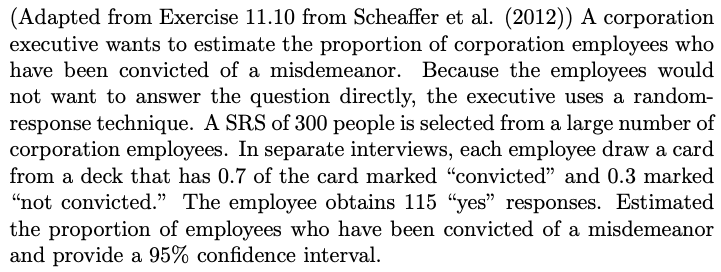
\includegraphics[width = 16cm]{img/Q1.png}
    %\caption{Section 6.1 Q8}
    %\label{fig:figure1label}
\end{figure}

\subsection*{Solution}

Let $\theta=0.7.$ And what we want to estimate is $p.$

Note that $P(Y)=115/300=\theta P(Y|C)+(1-\theta) P(Y|NC)
0.7 P(Y|C)+0.3 P(Y|NC).$

And note that $P(Y|C)=P(N|NC)=1-P(Y|NC).$

Therefore $115/300 = 0.7 P(Y|C) + 0.3 (1-P(Y|C)).$ We solve out 
$P(Y|C)=5/24.$

Hence $\hat{p}=P(Y|C)=5/24=0.2083.$

And its variance is 
$$\widehat{Var(\hat{p})}=\frac{1}{(2\theta -1)^2}(\frac{1}{n})P(Y)(1-P(Y))=4.9248\times 10^{-3}.$$

Therefore a proper 95\% C.I. for it can be 
$$(\hat{p} \pm t_{n-1,1-\frac{\alpha}{2}} \sqrt{\widehat{Var(\hat{p})}}~)=(0.2083 \pm 1.9679 \times 0.0702)=(0.2083 \pm 0.1381).$$


\newpage
\section{Q2}
\begin{figure}[htp]
    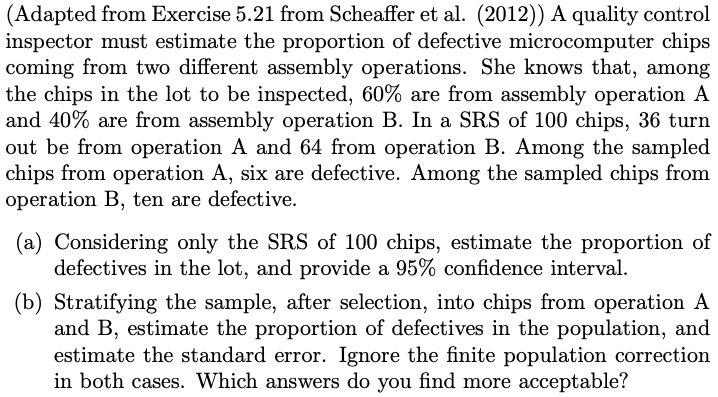
\includegraphics[width = 15cm]{img/Q2.png}
    %\caption{Section 6.1 Q8}
    %\label{fig:figure1label}
\end{figure}
\subsection*{Solution}
\subsection{(a)}
The point estimate should be $\hat{p}=\frac{6+10}{64+36}=\frac{16}{100}=0.16.$

And using $\widehat{Var(\hat{p})}=(1-\frac{n}{N})\frac{1}{n-1}\hat{p}(1-\hat{p})=1.3575\times 10^{-3}.$

Hence a proper 95\% C.I. for it should be $$(\hat{p} \pm t_{n-1,0.975}\sqrt{\widehat{Var(\hat{p})}}~)=(0.16 \pm 1.9842*0.0368)=(0.16 \pm 0.07301).$$

\subsection{(b)}
Use $\widehat{p_{pst}}=0.6*\frac{6}{36}+0.4*\frac{10}{64}=0.1625$ as the point estimate.


We stratify all the chips in the lot into 2 groups: from A and from B. 
Therefore $\hat{p_1}=\frac{6}{36}=\frac{1}{6}.$

And $\hat{p_2}=\frac{10}{64}=0.15625.$

Therefore, using $\hat{\sigma_i}^2=\frac{n_i}{n_i-1}\hat{p_i}(1-\hat{p_i}),$ one can
have $\hat{\sigma_1}^2=\frac{1}{7}.$ And $\hat{\sigma_2}^2=0.1339.$

Using the formulae 
$$\widehat{Var(\widehat{p_{pst}})}=\sum_{i=1}^{2}\frac{N-n}{nN}\frac{N_i}{N} \hat{\sigma_i}^2
+ \sum_{i=1}^2 \frac{1}{n^2}\frac{N-n}{N-1}(1-\frac{N_i}{N})\hat{\sigma_i}^2=1.4065*10^{-3}.$$

Then the s.e. is $\sqrt{1.4065*10^{-3}}=0.03750.$ 

And a 95\% C.I. for it should be $$(0.1625 \pm 1.96*0.0375) = (0.1625 \pm 0.0735).$$

I think the latter answer is more acceptable because I think the point estimate is more reasonable, 
while these two's variance are almost the same. The sample of things from opearation A is too few.


\newpage
\section{Q3}
\begin{figure}[htp]
    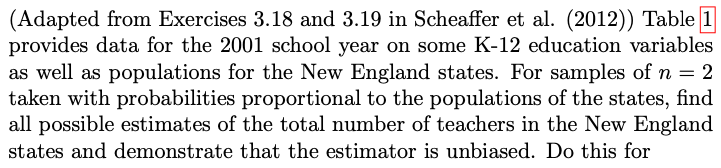
\includegraphics[width = 15cm]{img/Q3(1).png}
    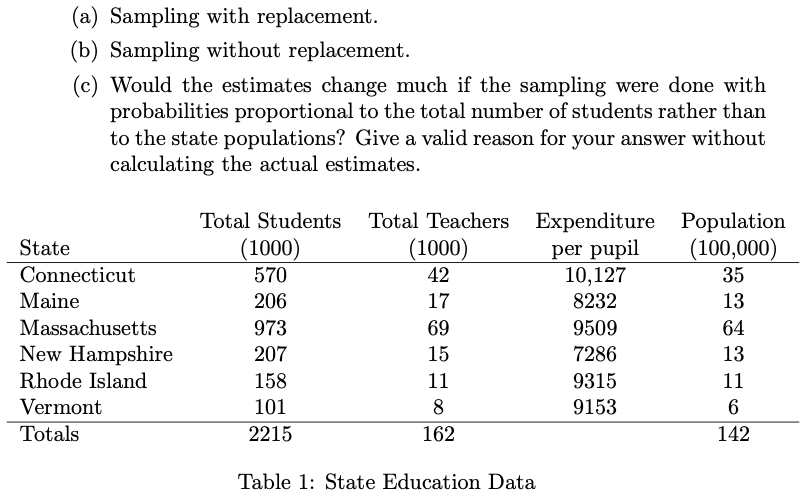
\includegraphics[width = 15cm]{img/Q3(2).png}
\end{figure}
\subsection*{Solution}

Index the 6 states with 

1: Connecticut; 

2: Maine; 

3: Massachusetts; 

4: New Hampshire; 

5: Rhode Island; 

6: Vermont.

And calculate the total population, which is $N=142.$

\subsection{(a)}

When applying the with replacement method, the probabilities of 
selection are "directly proportional to the populations of the states"
denoted as $\delta_i, i=1,2,\dots,6.$ Then we have 

$\delta_1 = 0.2465.$ $\delta_2 = 0.0915.$ $\delta_3 = 0.4507.$
$\delta_4 = 0.0915.$ $\delta_5 = 0.0775.$ $\delta_6 = 0.0423.$

With this, it can be easier for me to describe the $P_{WR}(i,j),$ 
which means the probability of $\{i,j\} (i,j \in \{1,2,3,4,5,6\})$
is being selected out. 

It is obvious that 
$$P_{WR}(i,j)=2\delta_i \delta_j, i\neq j,$$
$$P_{WR}(i,j)=\delta_i^2~~~, i = j.$$

Then we will have 

$P_{WR}(1,2)=0.0451.$ $P_{WR}(1,3)=0.2222.$ 
$P_{WR}(1,4)=0.0451.$ $P_{WR}(1,5)=0.0382.$

$P_{WR}(1,6)=0.0209.$ $P_{WR}(2,3)=0.0825.$
$P_{WR}(2,4)=0.0167.$ $P_{WR}(2,5)=0.0142.$

$P_{WR}(2,6)=0.0074.$ $P_{WR}(3,4)=0.0825.$
$P_{WR}(3,5)=0.0699.$ $P_{WR}(3,6)=0.0381.$

$P_{WR}(4,5)=0.0142.$ $P_{WR}(4,6)=0.0074.$
$P_{WR}(5,6)=0.0066.$ $P_{WR}(1,1)=0.0608.$

$P_{WR}(2,2)=0.0084.$ $P_{WR}(3,3)=0.2031.$
$P_{WR}(4,4)=0.0084.$ $P_{WR}(5,5)=0.0060.$

$P_{WR}(6,6)=0.0018.$

~\ 

Using the formulae 
$\widehat{\tau_{WR}}(i,j)=\frac{1}{2}(\frac{Y_i}{\delta_i}+\frac{Y_j}{\delta_j}),$
we can deduce that 

$\widehat{\tau_{WR}}(1,2)=178.12.$ 
$\widehat{\tau_{WR}}(1,3)=161.74.$
$\widehat{\tau_{WR}}(1,4)=176.16.$
$\widehat{\tau_{WR}}(1,5)=156.16.$

$\widehat{\tau_{WR}}(1,6)=179.76.$
$\widehat{\tau_{WR}}(2,3)=169.44.$
$\widehat{\tau_{WR}}(2,4)=174.86.$
$\widehat{\tau_{WR}}(2,5)=163.86.$

$\widehat{\tau_{WR}}(2,6)=187.46.$
$\widehat{\tau_{WR}}(3,4)=158.51.$
$\widehat{\tau_{WR}}(3,5)=147.52.$
$\widehat{\tau_{WR}}(3,6)=171.11.$

$\widehat{\tau_{WR}}(4,5)=152.93.$
$\widehat{\tau_{WR}}(4,6)=176.53.$
$\widehat{\tau_{WR}}(5,6)=165.53.$
$\widehat{\tau_{WR}}(1,1)=170.39.$

$\widehat{\tau_{WR}}(2,2)=185.79.$
$\widehat{\tau_{WR}}(3,3)=153.10.$
$\widehat{\tau_{WR}}(4,4)=163.93.$
$\widehat{\tau_{WR}}(5,5)=141.94.$

$\widehat{\tau_{WR}}(6,6)=189.13.$


Calculate that 
$$E[\widehat{\tau_{WR}}]
=\sum_{1\leq i\leq j\leq 6}P_{WR}(i,j)\widehat{\tau_{WR}(i,j)}
=162.13(=162).$$

Therefore it is unbiased.

\subsection{(b)}
Now we need to consider things without replacement. In this case 
we need to calculate $\pi_i.$ 

To calculate $P_{WOR}(i,j)$, we use the formulae 
$$P_{WOR}(i,j)=
\frac{m_i}{\sum_{k=1}^6 m_k} \frac{m_j}{\sum_{l \neq i} m_l}
+\frac{m_j}{\sum_{k=1}^6 m_k} \frac{m_i}{\sum_{l \neq j} m_l}.$$

Then we will have 

$P_{WOR}(1,2)=0.0548.$ $P_{WOR}(1,3)=0.3497.$ 
$P_{WOR}(1,4)=0.0548.$ $P_{WOR}(1,5)=0.0460.$

$P_{WOR}(1,6)=0.0247.$ $P_{WOR}(2,3)=0.1205.$
$P_{WOR}(2,4)=0.0185.$ $P_{WOR}(2,5)=0.0155.$

$P_{WOR}(2,6)=0.0083.$ $P_{WOR}(3,4)=0.1205.$
$P_{WOR}(3,5)=0.1014.$ $P_{WOR}(3,5)=0.0546.$

$P_{WOR}(4,5)=0.0155.$ $P_{WOR}(4,6)=0.0083.$
$P_{WOR}(5,6)=0.0070.$

~\ 

We need to calculate $\pi_i$, i.e., the probabilities of $i$-th 
cluster being selected in the sample. 
Using the formulae $$\pi_i = 
\delta_i + \sum_{j \neq i}\delta_j \delta_i/(1-\delta_j),$$ 
we can calculate that $\pi_1 = 0.53,
\pi_2 = 0.22, \pi_3 = 0.75, \pi_4 = 0.22, \pi_5 = 0.19, \pi_6 = 0.10.$



At this stage, we will calculate $\widehat{\tau_{WOR}(i,j)}$, 
using the formulae that 
$$\widehat{\tau_{WOR}(i,j)}=\frac{m_i}{\pi_i} + \frac{m_j}{\pi_j}.$$

Then we can have the result of 

$\widehat{\tau_{WOR}}(1,2)=157.37.$ 
$\widehat{\tau_{WOR}}(1,3)=171.25.$
$\widehat{\tau_{WOR}}(1,4)=147.43.$
$\widehat{\tau_{WOR}}(1,5)=137.14.$

$\widehat{\tau_{WOR}}(1,6)=159.25.$
$\widehat{\tau_{WOR}}(2,3)=169.27.$
$\widehat{\tau_{WOR}}(2,4)=145.45.$
$\widehat{\tau_{WOR}}(2,5)=135.17.$

$\widehat{\tau_{WOR}}(2,6)=157.27.$
$\widehat{\tau_{WOR}}(3,4)=160.18.$
$\widehat{\tau_{WOR}}(3,5)=149.89.$
$\widehat{\tau_{WOR}}(3,6)=172.$

$\widehat{\tau_{WOR}}(4,5)=126.08.$
$\widehat{\tau_{WOR}}(4,6)=148.18.$
$\widehat{\tau_{WOR}}(5,6)=137.89.$

~\ 

Calculate that 
$$E[\widehat{\tau_{WOR}}]
=\sum_{1\leq i < j\leq 6}P_{WOR}(i,j)\widehat{\tau_{WOR}(i,j)}
=161.35(=162).$$

\subsection{(c)}
I think the estimate would not change very much 
if the sampling were with respect
to the amount of students as the proportions 
of students' distribution are very similar to 
the proportions of the population.


\newpage
\section{Q4}
\begin{figure}[htp]
    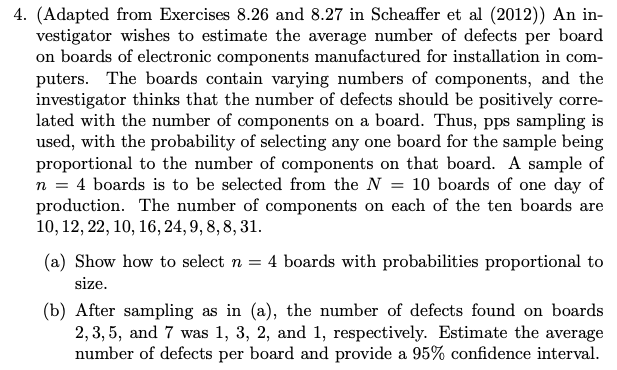
\includegraphics[width = 15cm]{img/Q4.png}
\end{figure}
\subsection*{Solution}

\subsection{(a)}
We label the boards with indices from 1 to 10.

Assign 1-10 to board 1. 
11-22 to board 2.
23-44 to board 3.
45-54 to board 4.
55-70 to board 5.
71-94 to board 6.
95-103 to board 7.
104-111 to board 8.
112-119 to board 9.
120-150 to board 10.

Then we randomly generate (e.g., using systematic sampling or using 
Excel) 4 integers inclusively between 1 and 150.

\subsection{(b)}
$N=10,n=4,M=150.$

We first calculate the $p_i$'s we need. We can know that 
$$p_1=12/150=0.08, p_2=22/150=0.1467, 
p_3=16/150=0.1067, p_4=9/150=0.06.$$
$$m_1=12,m_2=22,m_3=16, m_4=9.$$
$$Y_1=1,Y_2=3,Y_3=2,Y_4=1.$$

Then we need to calculate 
$$\hat{\tau_{pps}}=\frac{1}{n}\sum_{j=1}^n \frac{Y_i}{p_i}=17.09.$$

Then using the formulae 
$$\hat{\mu_{pps}}=\frac{1}{N} \hat{\tau_{pps}}=1.709.$$

And the $$\widehat{Var(\hat{\mu_{pps}})}
=\frac{1}{N^2n(n-1)} \sum_{i=1}^n (\frac{Y_i}{p_i}-\hat{\tau_{pps}})^2=0.0294.$$

$t_{n-1,1-\frac{\alpha}{2}}=qt(0.975,3)=3.182.$
Therefore, a 95\% C.I. for it should be 
$$( \hat{\mu_{pps}} \pm t_{n-1,1-\frac{\alpha}{2}} \sqrt{\widehat{Var(\hat{\mu_{pps}})}} ~)
=(1.709 \pm 3.182* 0.1715 )=(1.709 \pm 0.5456)=(1.1634,2.2546).$$
















\end{document}
